\section{Event selection}
\label{sec:selection}

\subsection{Signal region selection}
\label{sec:selection_sr}
Signal region events are selected using triggers with thresholds of 120\GeV on both \ptmisstrig~and \mhttrig.
The \ptmisstrig~corresponds to the magnitude of the vector \ptvec sum of all the PF candidates reconstructed at the trigger level, 
while the \mhttrig~is computed as the magnitude of the vector \ptvec sum of jets with $\pt > 20\GeV$ and $|\eta| < 5.0$ reconstructed 
at the trigger level. The energy fraction attributed to neutral hadrons in these jets is required to be smaller than 0.9. 
This requirement suppresses anomalous events with jets originating from detector noise. 
To be able to use the same triggers for selecting events in the muon control samples used for background prediction, muon candidates are not included in the \ptmisstrig~nor \mhttrig~computation. 
The trigger efficiency is measured to be $96\%$ for events passing the analysis selection for $\ptmiss > 250\GeV$ and becomes more than $99\%$ efficient for events with $\ptmiss > 350\GeV$.

Candidate events are required to have $\ptmiss > 250\GeV$. 
The leading AK4 jet in the signal event is required to have $ \pt > 80\GeV $ and $|\eta| < 4.7$, and the subleading AK4 jet is 
required to have $ \pt > 40\GeV$ and $|\eta| < 4.7$. In addition, if the leading jet is within the tracker range, $|\eta| < 2.5$,
it is required to have at least 10\% of its energy coming from charged particles and less than 80 \% of its energy attributed to 
neutral hadrons, as discussed in section~\ref{sec:objects}. This selection helps to remove events originating from beam-induced backgrounds. 
In addition, the analysis employs various event filters to reduce events with large misreconstructed \ptmiss~\cite{Sirunyan:2019kia} originating from noncollision backgrounds.

For the VBF signal events, two leading jets in opposite hemispheres are expected, with large dijet mass. Furthermore, these jets are 
expected to have large rapidity seperation and small azimuthal seperation. Therefore, this analysis employs several requirements on 
\mjj, \detajj and \dphijj, which can be found in Table~\ref{tab:selection}.

The main background processes in this search are the \Zvvjets and \Wlvjets processes. The \Zvvjets process is an irreducible 
background and constitutes the largest background in the search. In contrast, the background from \Wlvjets is suppressed by 
imposing a veto on events containing one or more loose muons or electrons with $ \pt >10\GeV$, or hadronically decaying $\tau$ 
leptons with $\pt>18\GeV$. Events that contain a loose, isolated photon with $\pt>15\GeV$ and $|\eta| < 2.5$ are also rejected. 
This helps to suppress electroweak (EW) backgrounds in which a photon is radiated from the initial state.
To reduce the contamination from top quark backgrounds, events are rejected if they contain a b tagged jet with $\pt > 20\GeV$ 
and $|\eta| < 2.4$. These jets are identified using the DeepCSV algorithm~\cite{CMS_NOTE_2018-323,Sirunyan:2017ezt}, 
adopting the ``medium'' working point, which corresponds to correctly identifying a jet originating from a bottom quark with 
a probability of 80\% and misidentifying a jet originating from a charm quark (light-flavor jet) with a probability of 12 (2)\%. 
Lastly, QCD multijet background with \ETm arising from mismeasurements of the jet momenta is suppressed by requiring the minimum
azimuthal angle between the \ptvecmiss direction and each of the first four leading jets with \pt greater than 30\GeV 
and $|\eta| < 2.4$ to be larger than 0.5 radians.

The selection requirements for this analysis are summarized in Table~\ref{tab:selection}.

{\color{gray}
The $N$-subjettiness variable $\tau_N$~\cite{Thaler:2010tr}
is also employed to further isolate jets arising from hadronic decays of $\PW$ or $\PZ$ bosons.
This observable measures the distribution of jet constituents relative to candidate subjet axes in order to quantify
how well the jet can be divided into $N$ subjets. Therefore, the ratio of the `2-subjettiness' to
the `1-subjettiness' ($\tau_2 / \tau_1$) has excellent capability for distinguishing jets
originating from boosted vector bosons from jets originating from light quarks and gluons.
The pruned jet mass and $N$-subjettiness requirements, whose use if referred to as $\PV$ tagging, result in a
70\% efficiency for tagging jets originating from $\PV$ bosons and a 5\% probability of misidentifying a jet as a $\PV$ jet.
Events that do not qualify for the mono-$\PV$ category are assigned to the monojet category. 
\begin{table*}[htb]
    \topcaption{Summary of the common selection requirements}
    \begin{center}
        \renewcommand{\arraystretch}{1}
        \ifthenelse{\boolean{cms@external}}{\footnotesize}{\resizebox{\textwidth}{!}}
        {
            \begin{scotch}{l c c}
                Variable                           & Selection                       & Target background \\
                \hline
                Muon (electron) veto               & $\pt > 10\GeV,~|\eta| < 2.4 (2.5)$  & \Zlljets,~\Wlvjets \\
                $\tau$ lepton veto                 & $\pt > 18\GeV,~|\eta| < 2.3$        & \Zlljets,~\Wlvjets  \\
                Photon veto                        & $\pt > 15\GeV,~|\eta| < 2.5$        & \phojets \\
                Bottom jet veto                    & DeepCSV medium $< 0.4941 / 0.4184$ (2017 / 2018) &  Top quark\\
                                                   & for all jets with $\pt > 20\GeV,~|\eta| < 2.4$ &\\
                $\ptmiss$                          & ${>} 250\GeV$                          & QCD, top quark, \Zlljets \\
                $\Delta\phi$($\ptvecjet$,$\ptvecmiss$)   &  $ {>} 0.5$ radians               & QCD \\
                Leading AK4 jet $\pt$ and $\eta$   & ${>} 80\GeV$ and $ |\eta| < 4.7$      & All \\
                Subleading AK4 jet $\pt$ and $\eta$   & ${>} 40\GeV$ and $ |\eta| < 4.7$      & All \\
                $\mjj$                               & $> 200\GeV$         
                $\detajj$                            & $> 1.0$
                $\dphijj$                            & $< 1.5$
            \end{scotch}
        }
        \label{tab:selection}
    \end{center}
\end{table*}

Fig.~\ref{fig:SR_pre_monojet_2017}, ~\ref{fig:SR_pre_monoV_2017},~\ref{fig:SR_pre_monojet_2018}, ~\ref{fig:SR_pre_monoV_2018},
shows the distribution of the \ETmiss, the number of
jets, $\pt$ and $\eta$ distribution of the leading AK4 jet for events
in the monojet and mono-V signal categories respectively for 2017 and 2018 datasets.

\begin{figure}[htbp]
    \begin{center}
        
\includegraphics[width=0.49\textwidth]{fig/placeholder.png}
        
\includegraphics[width=0.49\textwidth]{fig/placeholder.png} \\
        
\includegraphics[width=0.49\textwidth]{fig/placeholder.png}
        
\includegraphics[width=0.49\textwidth]{fig/placeholder.png}
    \end{center}
    \caption{Comparison between data and monte carlo simulation in the monojet signal region for
        the recoil distribution, the AK4 jet multiplicity distribution,  $p_T$ and $\eta$
        distribution of the leading AK4  jet in 2017 dataset.}
    \label{fig:SR_pre_monojet_2017}
\end{figure}

\begin{figure}[htbp]
    \begin{center}
        
\includegraphics[width=0.49\textwidth]{fig/placeholder.png}
        
\includegraphics[width=0.49\textwidth]{fig/placeholder.png} \\
        
\includegraphics[width=0.49\textwidth]{fig/placeholder.png}
        
\includegraphics[width=0.49\textwidth]{fig/placeholder.png}
    \end{center}
    \caption{Comparison between data and monte carlo simulation in the monojet signal region for
        the recoil distribution, the AK4 jet multiplicity distribution,  $p_T$ and $\eta$
        distribution of the leading AK4  jet in 2017 dataset.}
    \label{fig:SR_pre_monoV_2017}
\end{figure}

\begin{figure}[htbp]
    \begin{center}
        
\includegraphics[width=0.49\textwidth]{fig/placeholder.png}
        
\includegraphics[width=0.49\textwidth]{fig/placeholder.png} \\
        
\includegraphics[width=0.49\textwidth]{fig/placeholder.png}
        
\includegraphics[width=0.49\textwidth]{fig/placeholder.png}
    \end{center}
    \caption{Comparison between data and monte carlo simulation in the monojet signal region for
        the recoil distribution, the AK4 jet multiplicity distribution,  $p_T$ and $\eta$
        distribution of the leading AK4  jet in 2017 dataset.}
    \label{fig:SR_pre_monojet_2018}
\end{figure}

\begin{figure}[htbp]
    \begin{center}
        
\includegraphics[width=0.49\textwidth]{fig/placeholder.png}
        
\includegraphics[width=0.49\textwidth]{fig/placeholder.png} \\
        
\includegraphics[width=0.49\textwidth]{fig/placeholder.png}
        
\includegraphics[width=0.49\textwidth]{fig/placeholder.png}
    \end{center}
    \caption{Comparison between data and monte carlo simulation in the monojet signal region for
        the recoil distribution, the AK4 jet multiplicity distribution,  $p_T$ and $\eta$
        distribution of the leading AK4  jet in 2017 dataset.}
    \label{fig:SR_pre_monoV_2018}
\end{figure}

\newpage

\subsection{Single muon control region selection}
\label{sec:selection_cr_1m}

Single-muon control sample events are selected using full signal region criteria of VBF selection with the exception of the muon veto. 
The \ptmiss requirement is replacement an identical requirement on the hadronic recoil, which is defined as the sum of \ptvecmiss and the muon \vpt, 
and thus corresponds to the distribution of the W \pt.
In the single-muon control sample, exactly one tightly identified, isolated muon with $\pt > 20$~\GeV is required. 
No additional loose muons or electrons with $\pt > 10$~\GeV are allowed.
In addition, the transverse mass of the muon-$\vec p_{\rm T}^{\rm miss}$ system is required to be smaller than than 160~\GeV.
The transverse mass (\mt) is computed as $\mt = \sqrt{2\MET \pt^{\mu} (1 - \mathrm{cos}\Delta\phi)}$, 
where $\pt^{\mu}$ is the \pt of the muon, and $\Delta\phi$ is the angle between $\ptvec^{\mu}$ and $\ptvecmiss$.


Figs.~\ref{fig:SM_vbfhinv_2017} and~\ref{fig:SM_vbfhinv_2018} show the distributions of the recoil, 
the number of jets, and the $\pt$ and $\eta$ distribution of the leading AK4 jet
for events in the single-muon control sample for the VBF category in 2017 and 2018 datasets, respectively. 
Figs.~\ref{fig:SM_2_vbfhinv_2017} and~\ref{fig:SM_2_vbfhinv_2018} show the distributions of the leading muon \pt and $\eta$, 
as well as the muon-\ptmiss transverse mass, again for 2017 and 2018, respectively.


\begin{figure}[htbp]
    \begin{center}
        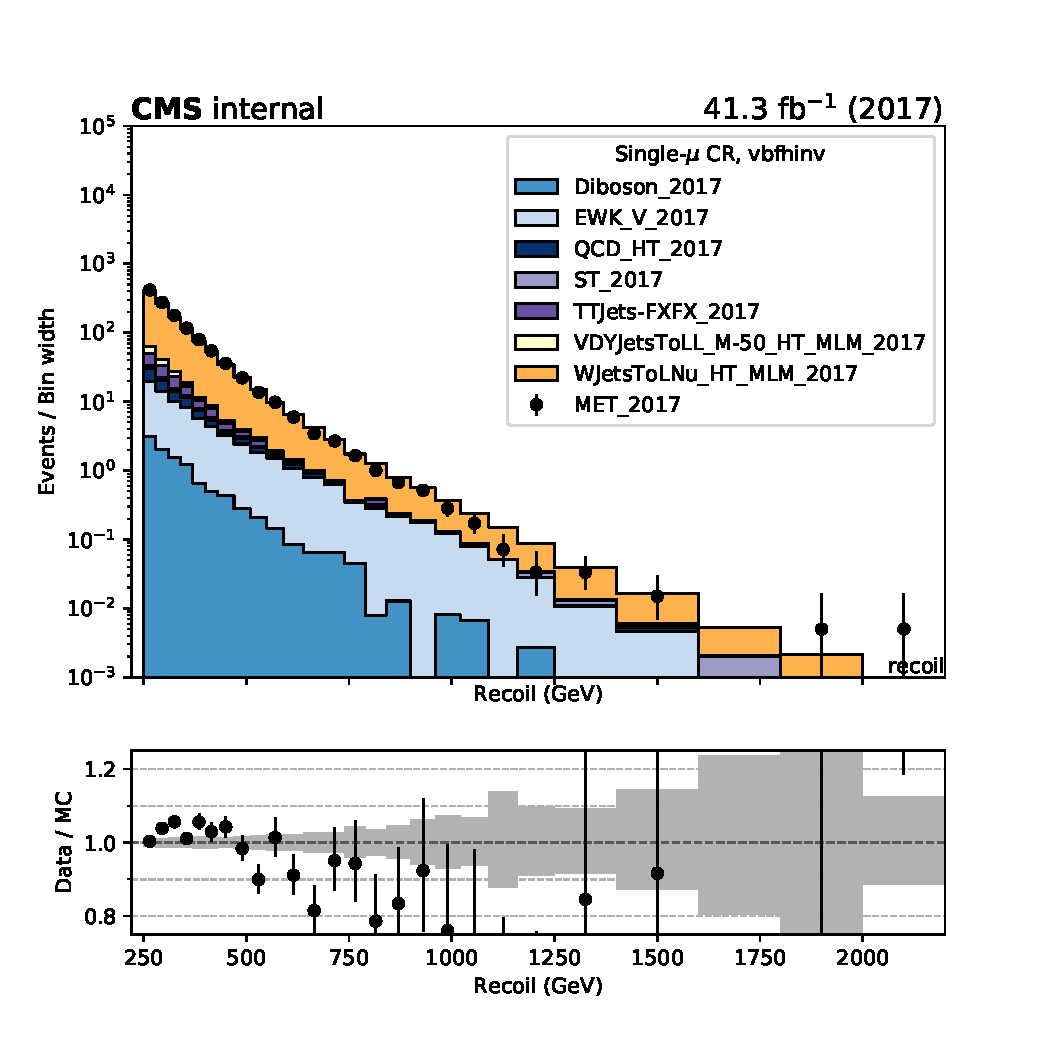
\includegraphics[width=0.49\textwidth]{fig/datamc/cr_1m_vbf/cr_1m_vbf_recoil_losf_2017.pdf}
        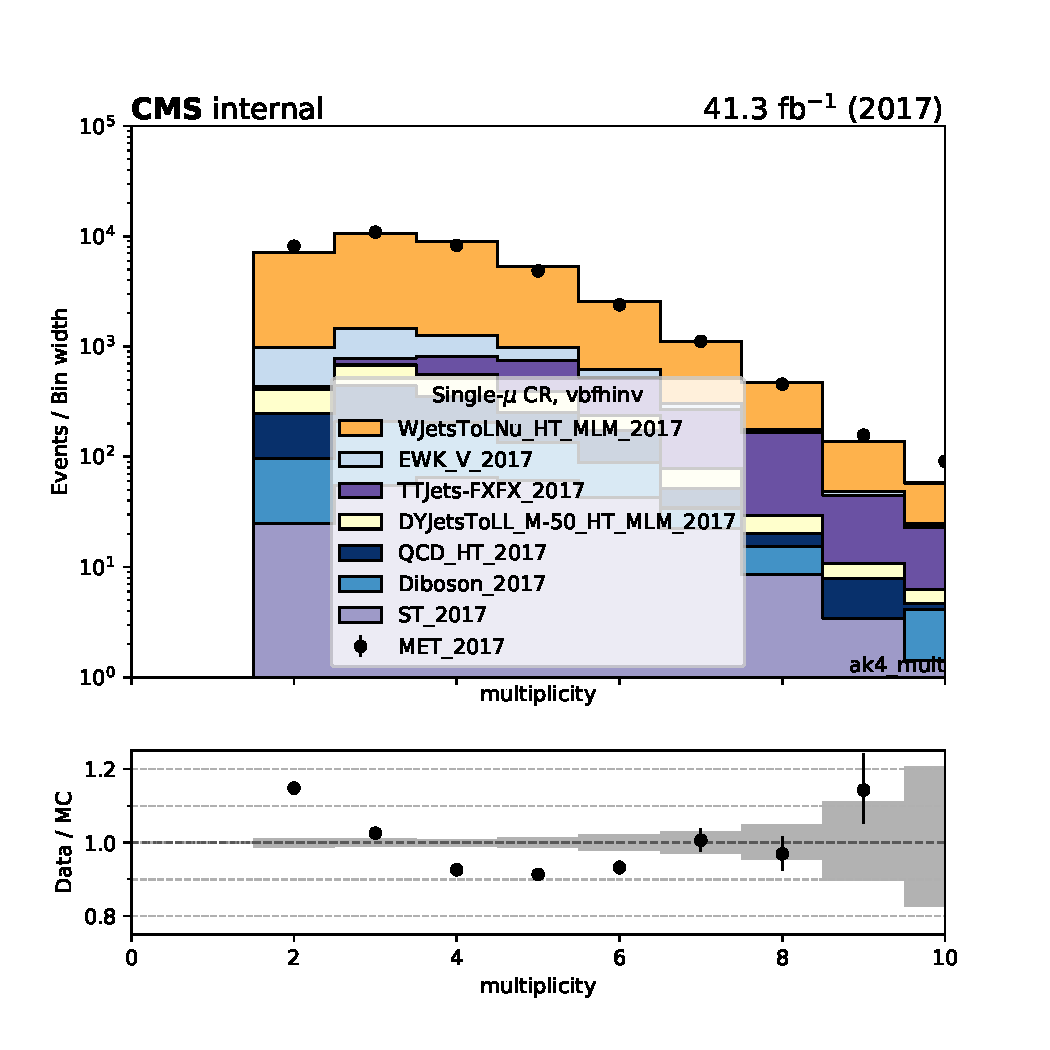
\includegraphics[width=0.49\textwidth]{fig/datamc/cr_1m_vbf/cr_1m_vbf_ak4_mult_losf_2017.pdf} \\
        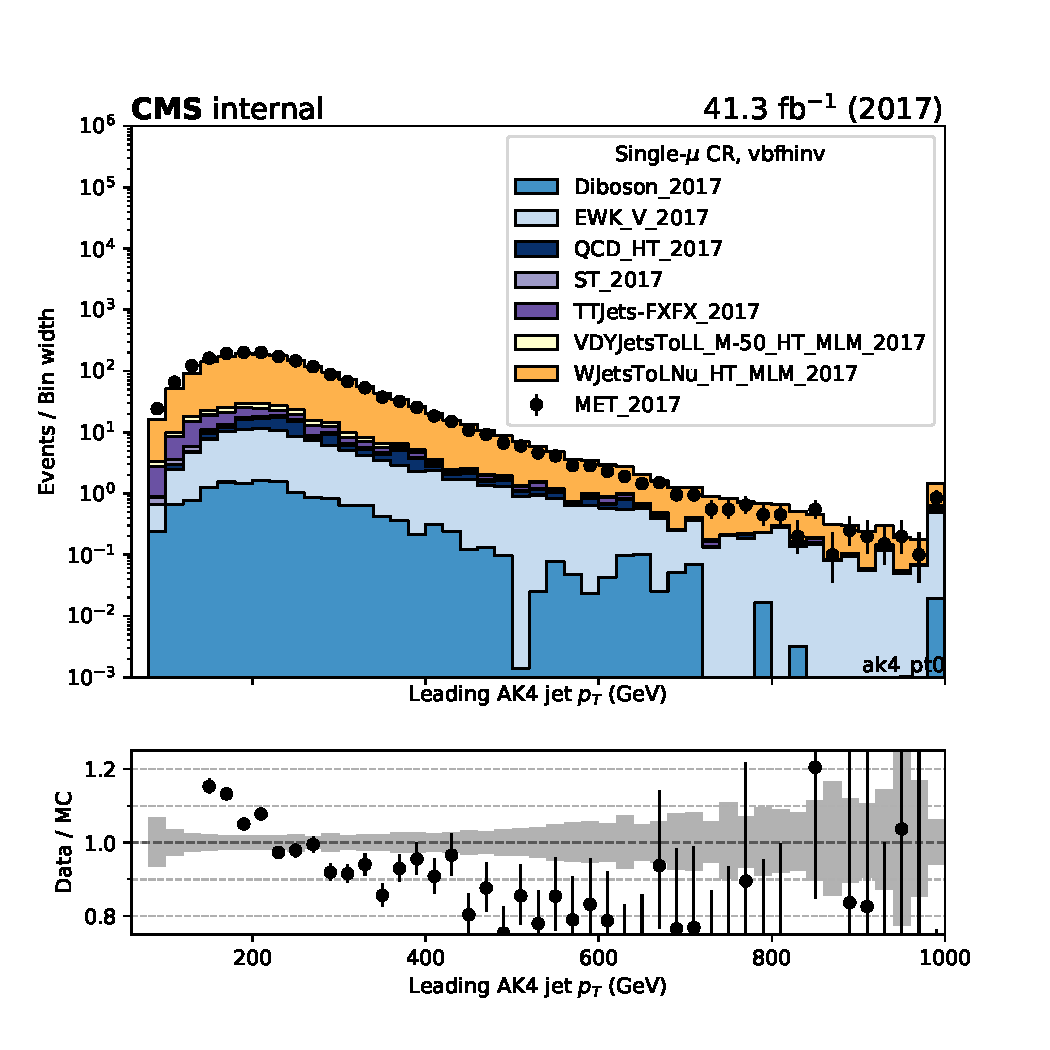
\includegraphics[width=0.49\textwidth]{fig/datamc/cr_1m_vbf/cr_1m_vbf_ak4_pt0_losf_2017.pdf}
        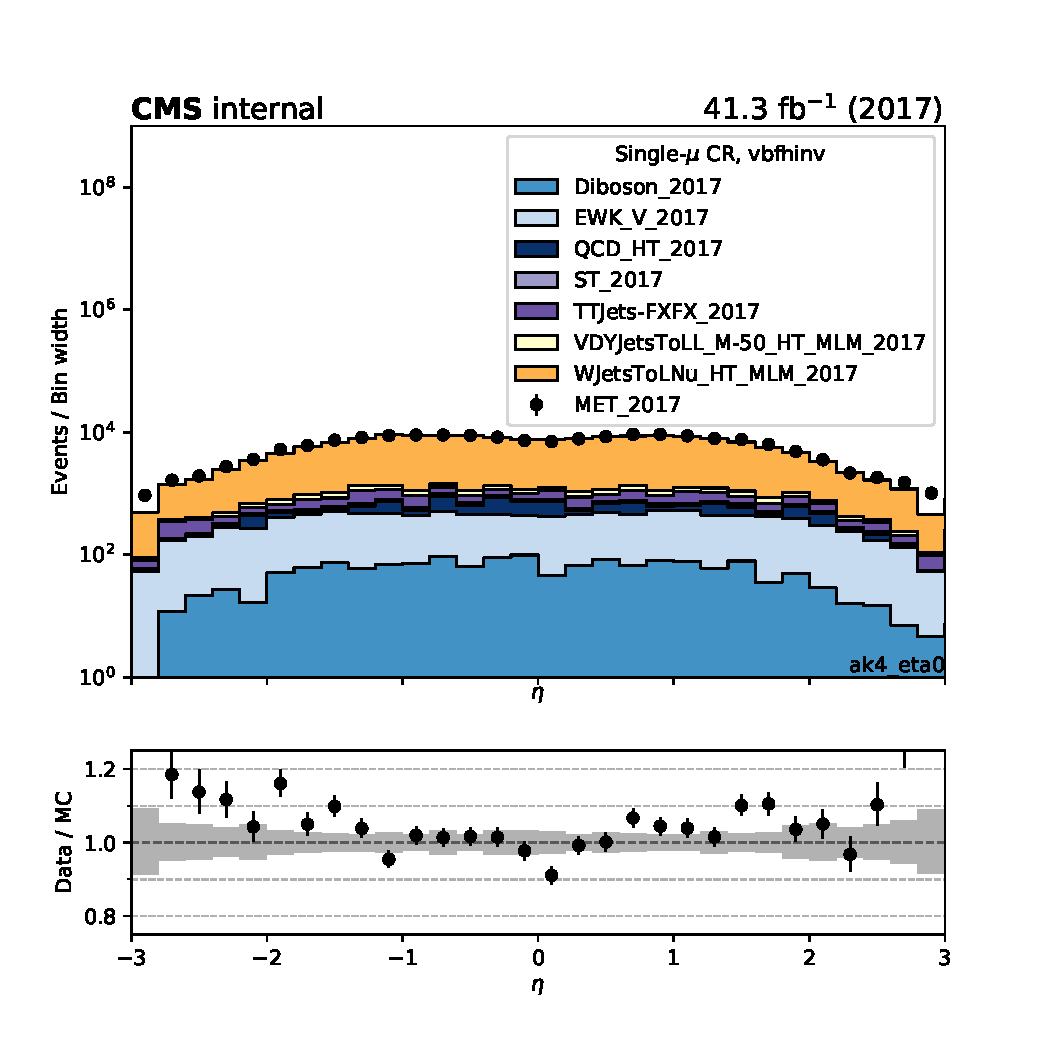
\includegraphics[width=0.49\textwidth]{fig/datamc/cr_1m_vbf/cr_1m_vbf_ak4_eta0_losf_2017.pdf}
    \end{center}
    \caption{Comparison between 2017 data and Monte Carlo simulation in the single muon control sample for
        the recoil distribution, the AK4 jet multiplicity distribution,  $\pt$ and $\eta$ distribution
        of the leading AK4 jet with the VBF selection.}
    \label{fig:SM_vbfhinv_2017}
\end{figure}

\begin{figure}[htbp]
    \begin{center}
        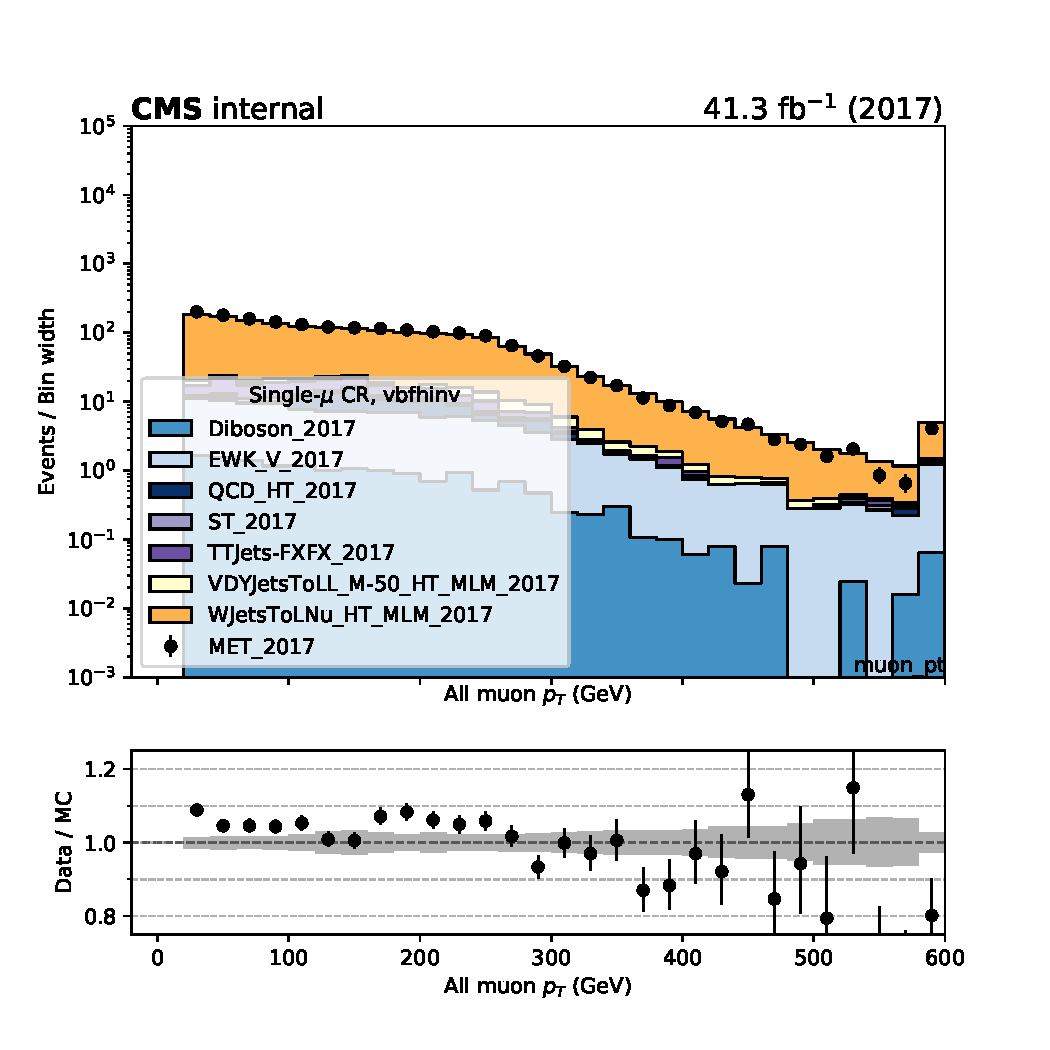
\includegraphics[width=0.49\textwidth]{fig/datamc/cr_1m_vbf/cr_1m_vbf_muon_pt_losf_2017.pdf}
        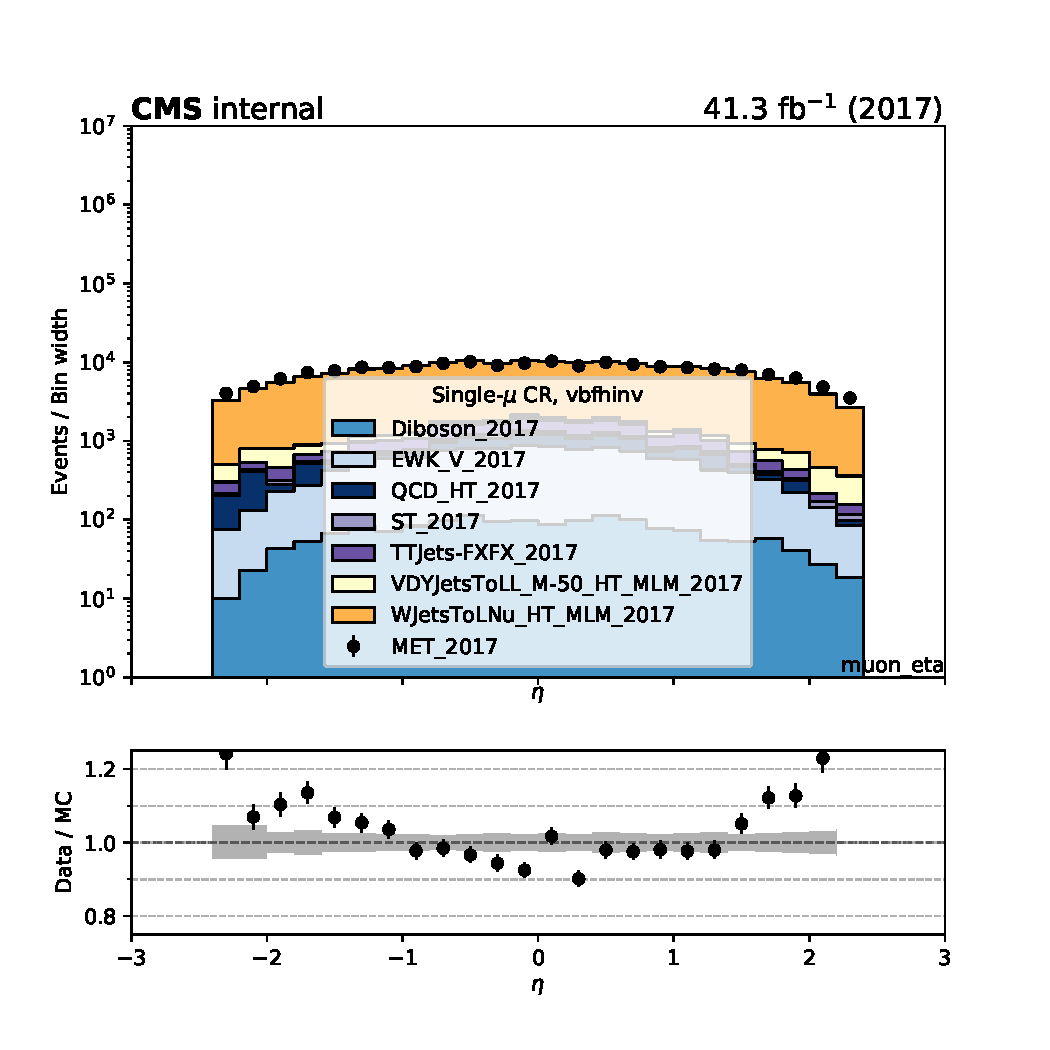
\includegraphics[width=0.49\textwidth]{fig/datamc/cr_1m_vbf/cr_1m_vbf_muon_eta_losf_2017.pdf} \\
        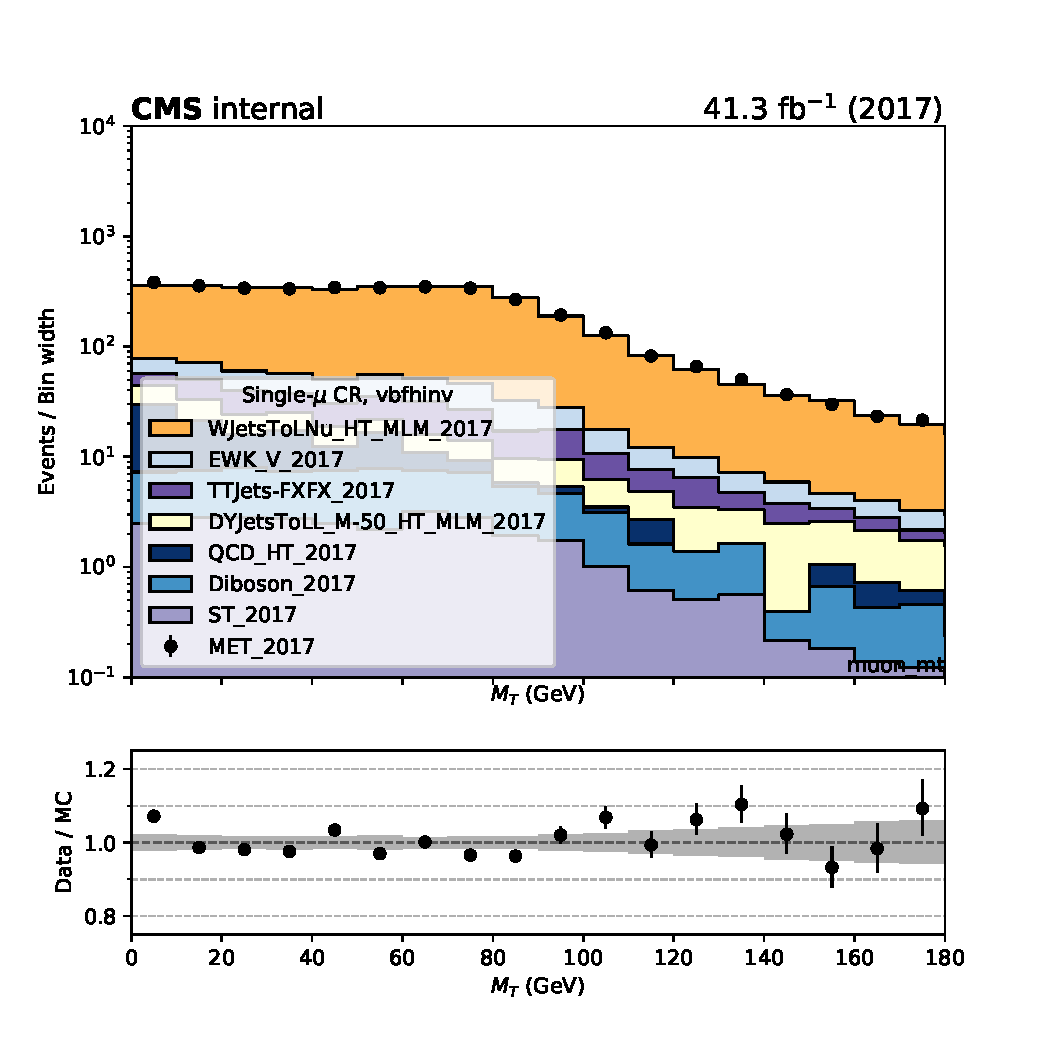
\includegraphics[width=0.49\textwidth]{fig/datamc/cr_1m_vbf/cr_1m_vbf_muon_mt_losf_2017.pdf}
    \end{center}
    \caption{Comparison between 2017 data and Monte Carlo simulation in the single muon control sample for
        the $\pt$ and $\eta$ of the leading muon and the transverse mass distribution with the VBF selection.}
    \label{fig:SM_2_vbfhinv_2017}
\end{figure}

\begin{figure}[htbp]
    \begin{center}
        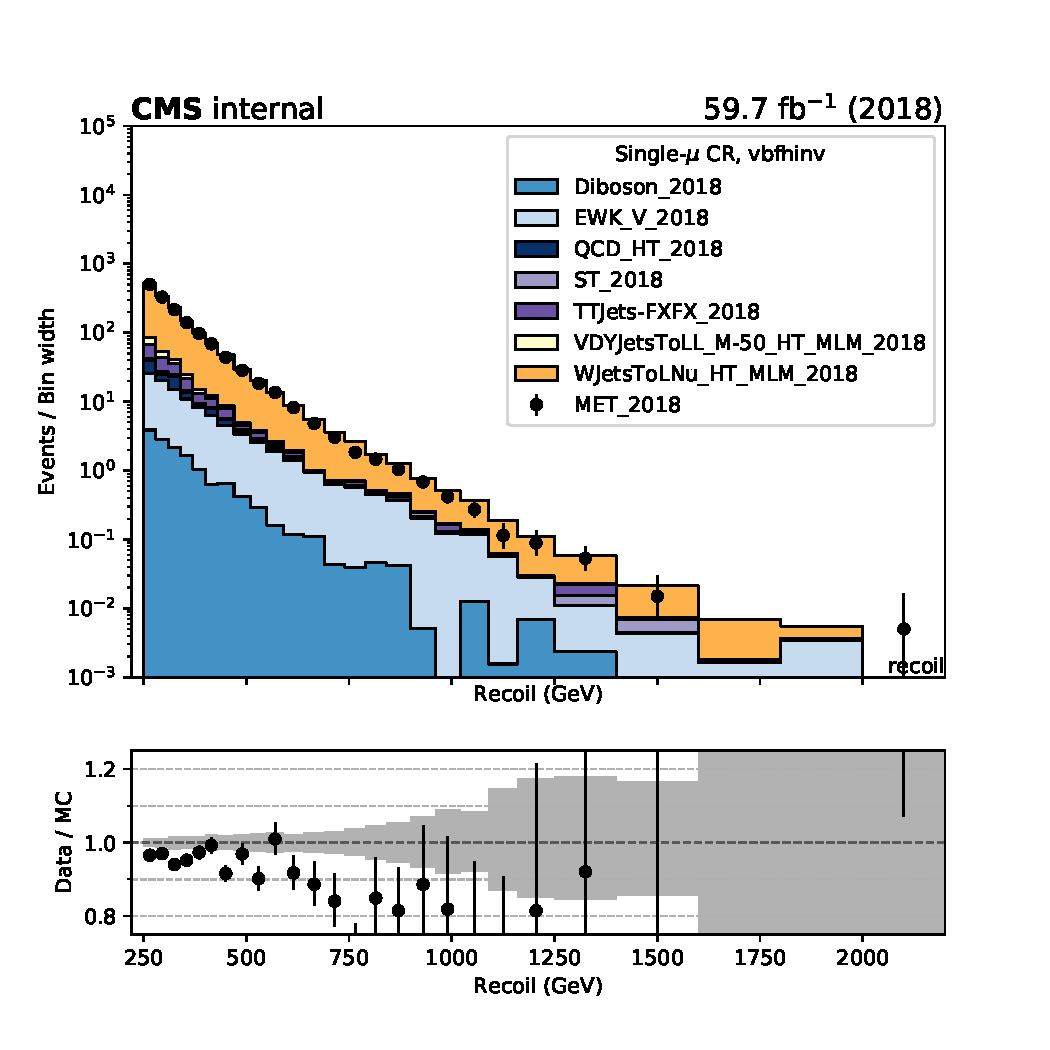
\includegraphics[width=0.49\textwidth]{fig/datamc/cr_1m_vbf/cr_1m_vbf_recoil_losf_2018.pdf}
        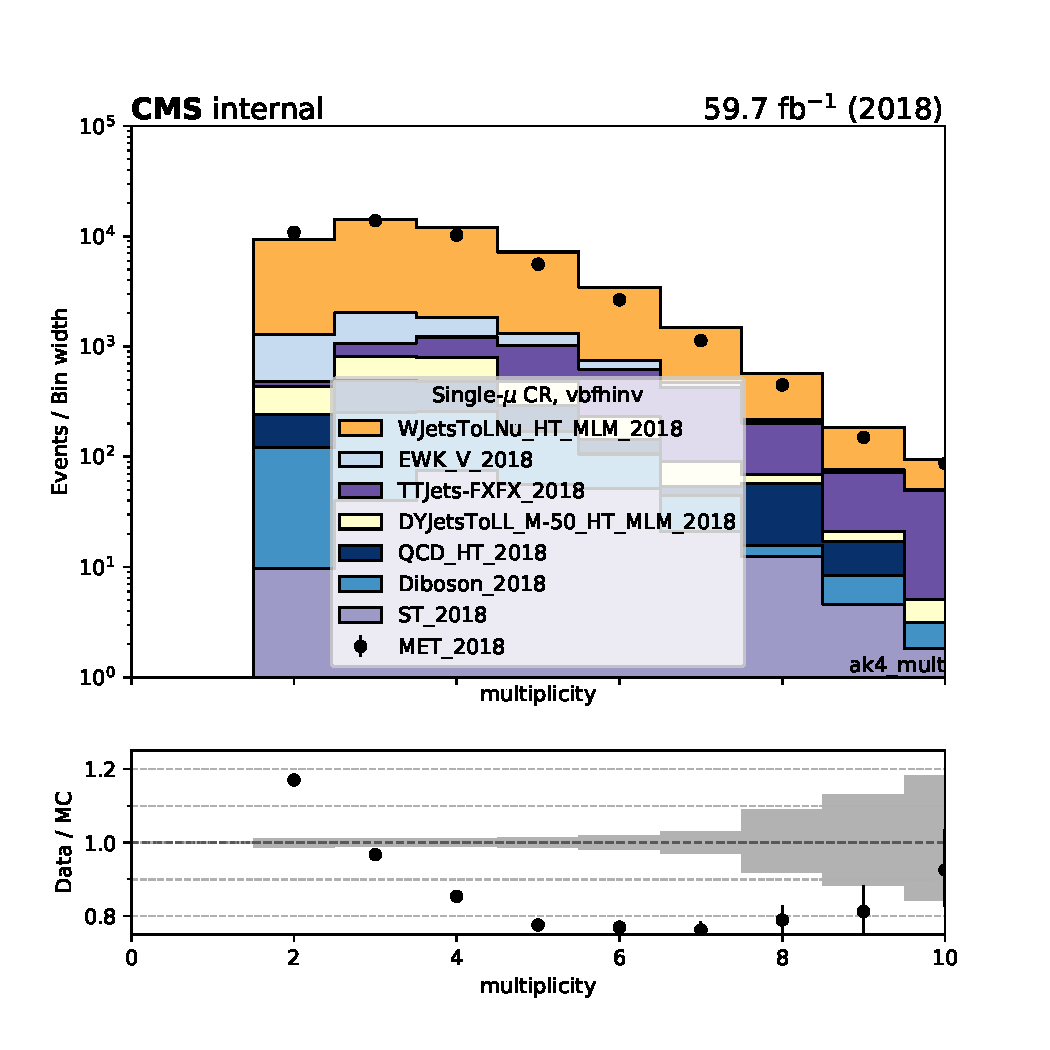
\includegraphics[width=0.49\textwidth]{fig/datamc/cr_1m_vbf/cr_1m_vbf_ak4_mult_losf_2018.pdf} \\
        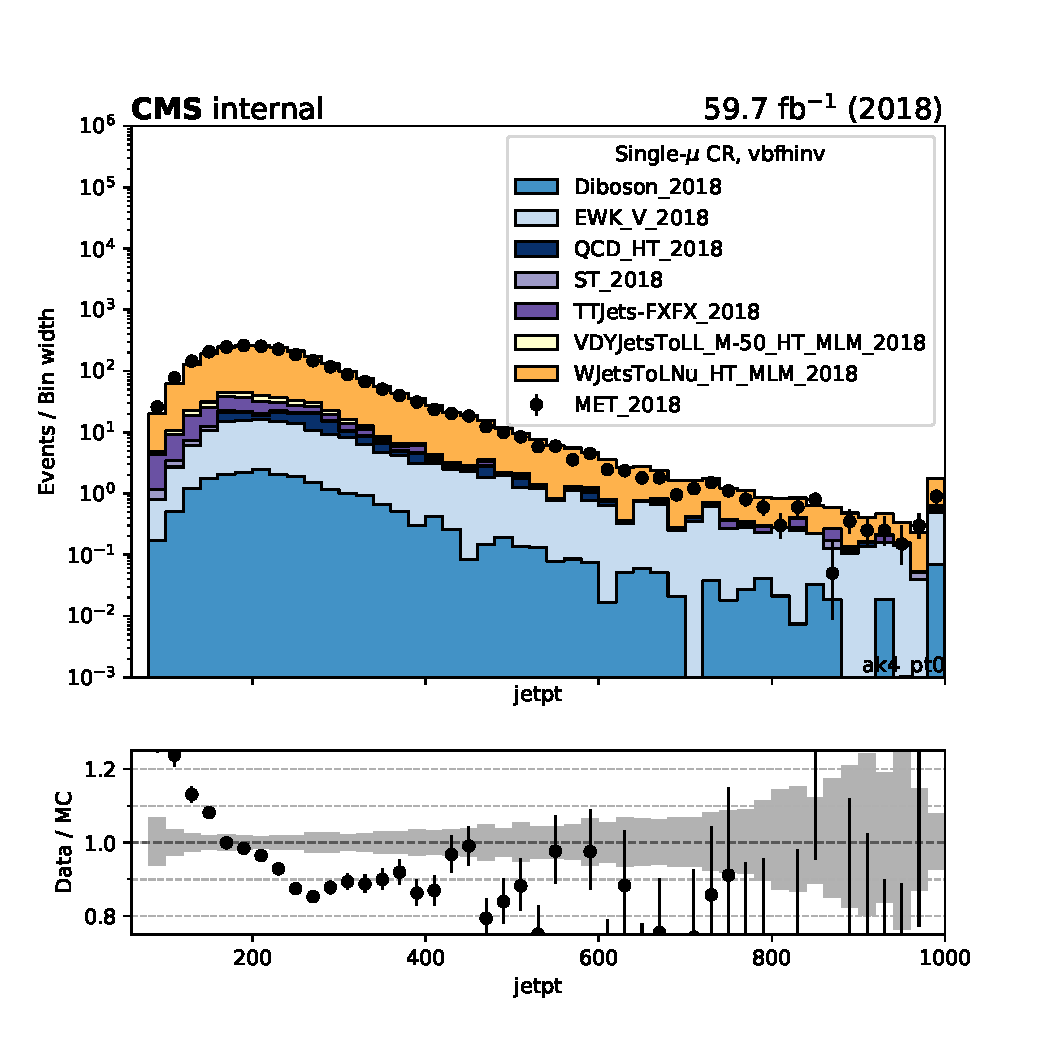
\includegraphics[width=0.49\textwidth]{fig/datamc/cr_1m_vbf/cr_1m_vbf_ak4_pt0_losf_2018.pdf}
        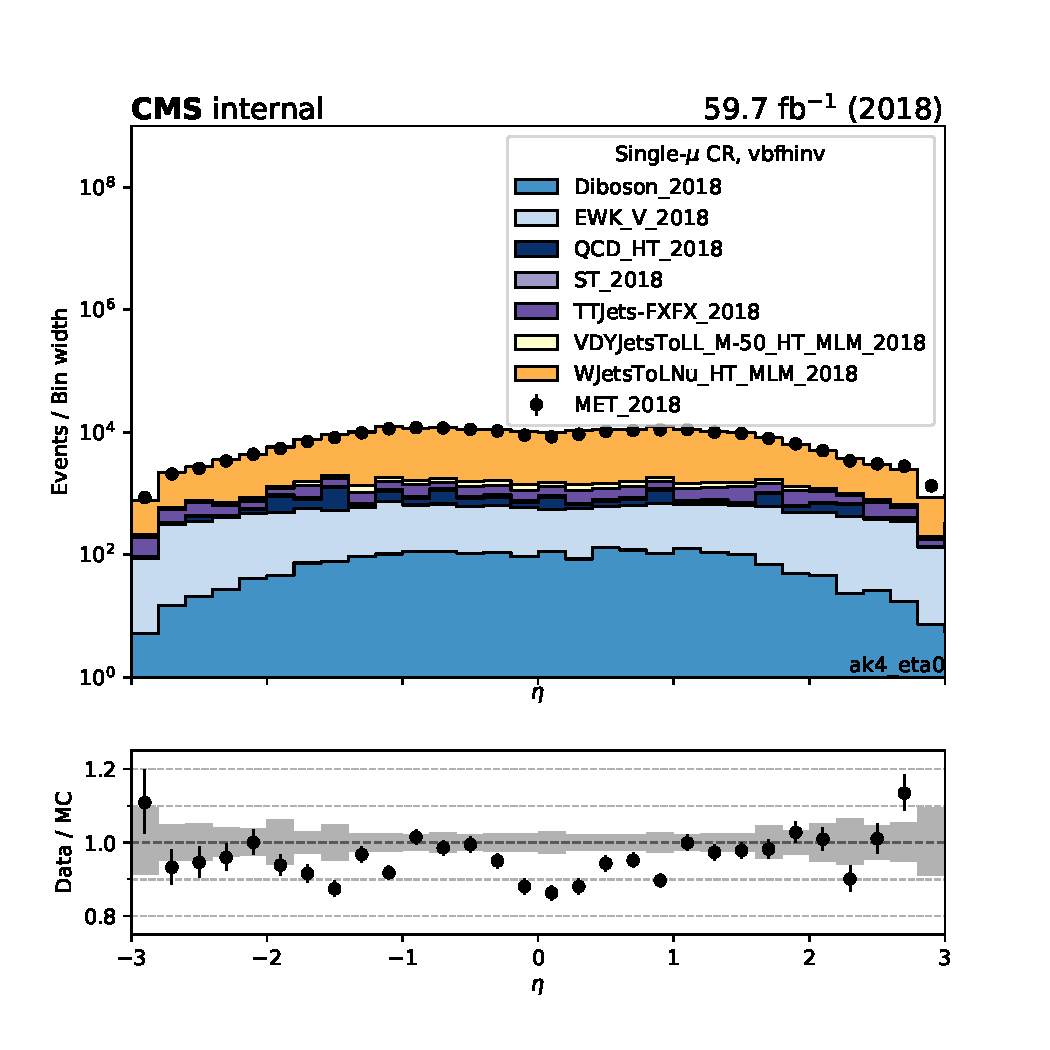
\includegraphics[width=0.49\textwidth]{fig/datamc/cr_1m_vbf/cr_1m_vbf_ak4_eta0_losf_2018.pdf}
    \end{center}
    \caption{Comparison between 2018 data and Monte Carlo simulation in the single muon control sample for
        the recoil distribution, the AK4 jet multiplicity distribution,  $\pt$ and $\eta$ distribution
        of the leading AK4 jet with the VBF selection.}
    \label{fig:SM_vbfhinv_2018}
\end{figure}

\begin{figure}[htbp]
    \begin{center}
        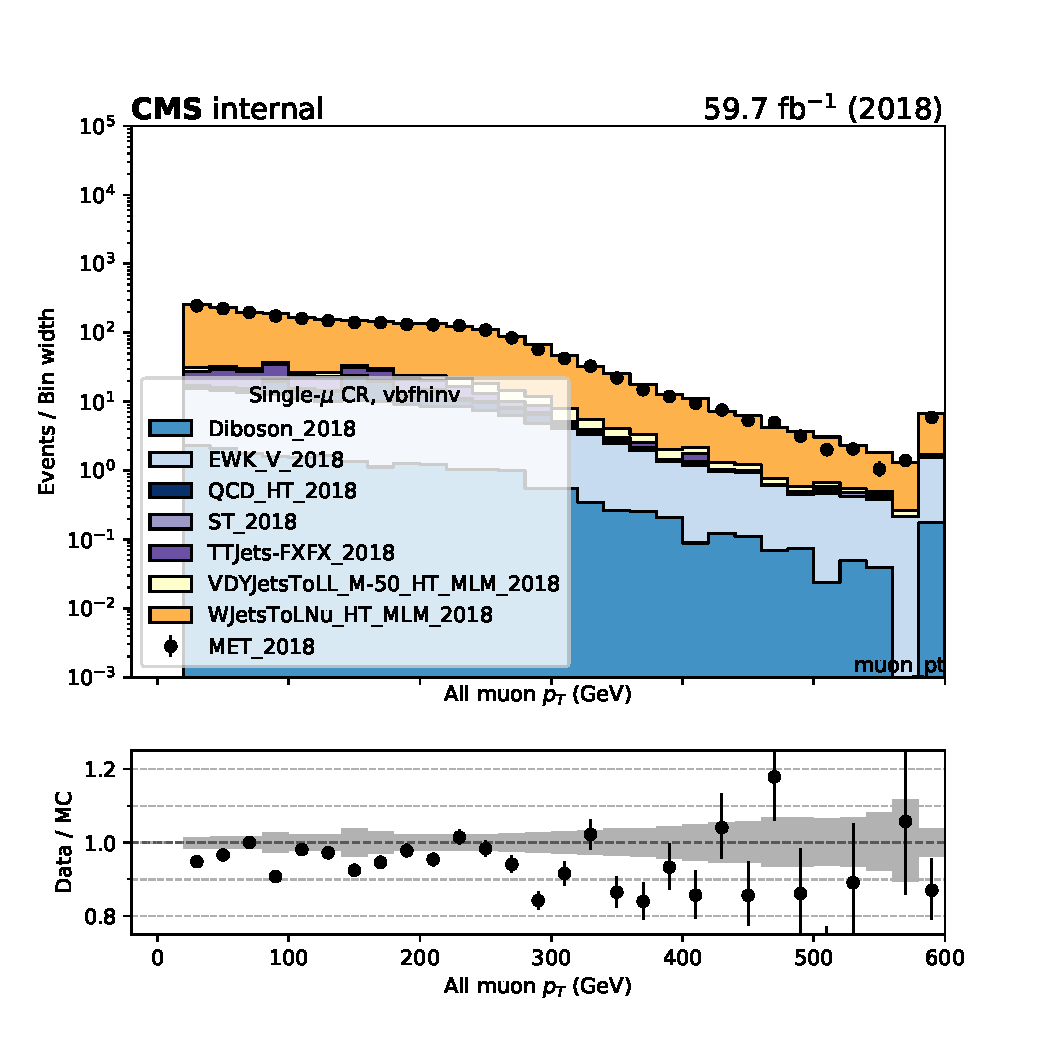
\includegraphics[width=0.49\textwidth]{fig/datamc/cr_1m_vbf/cr_1m_vbf_muon_pt_losf_2018.pdf}
        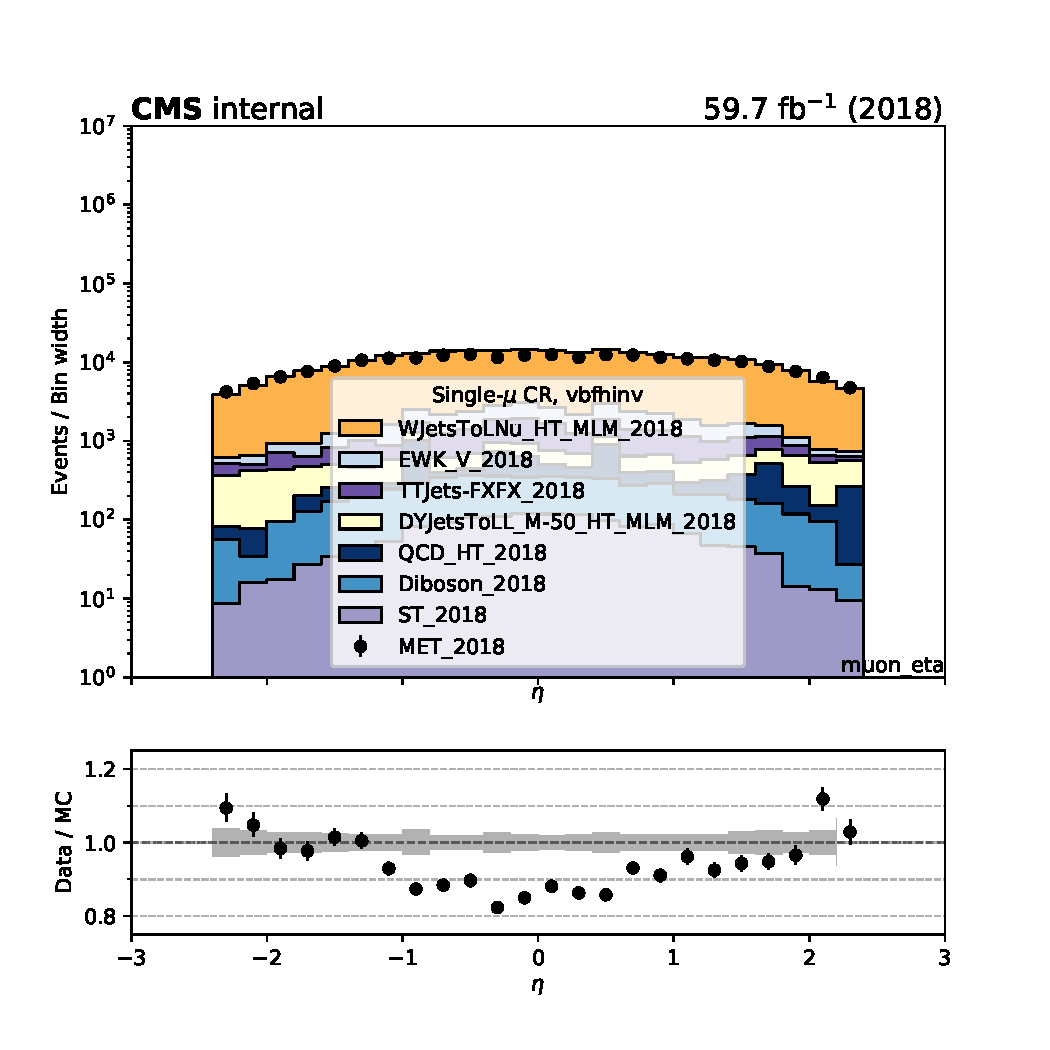
\includegraphics[width=0.49\textwidth]{fig/datamc/cr_1m_vbf/cr_1m_vbf_muon_eta_losf_2018.pdf} \\
        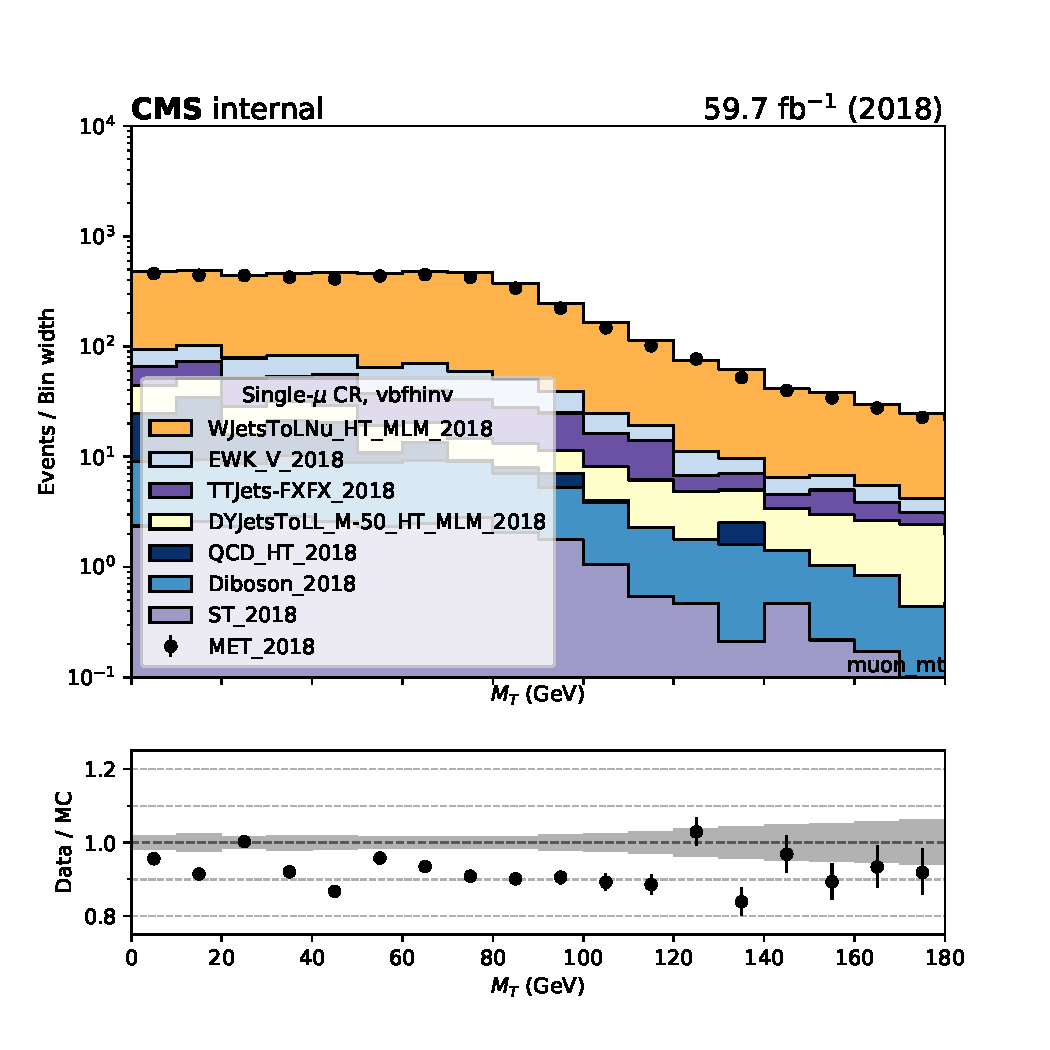
\includegraphics[width=0.49\textwidth]{fig/datamc/cr_1m_vbf/cr_1m_vbf_muon_mt_losf_2018.pdf}
    \end{center}
    \caption{Comparison between 2018 data and Monte Carlo simulation in the single muon control sample for
        the $\pt$ and $\eta$ of the leading muon and the transverse mass distribution with the VBF selection.}
    \label{fig:SM_2_vbfhinv_2018}
\end{figure}

\newpage

\subsection{Single electron control region selection}
\label{sec:selection_cr_1e}
Events for the single-electron control sample are collected with the single-electron and photon triggers described in Sec.~\ref{sec:samples}.  The \ptmiss requirement is replacement an identical requirement on the hadronic recoil, which is defined as the sum of \ptvecmiss and the electron \vpt, and thus corresponds to the distribution of the W \pt.
The events in the single-electron control sample are required to contain exactly one tightly identified and isolated electron with $\pt > 40$~\GeV.
In addition, the contamination from QCD multijet events in this control sample is suppressed by requiring \MET$ > 50$~\GeV and $\mt < 160 \GeV$.

Figs.~\ref{fig:SE_monojet_2017} and~\ref{fig:SE_monojet_2018} show the distributions of the recoil, the number of jets, and the $\pt$ and $\eta$ distribution of the leading AK4  jet
for events in the single-electron control sample for the monojet category in 2017 and 2018 datasets, respectively. Figs.~\ref{fig:SE_2_monojet_2017} and~\ref{fig:SE_2_monojet_2018} show the distributions of the leading electron \pt and $\eta$, as well as the electron-\ptmiss transverse mass, again for 2017 and 2018, respectively.

\begin{figure}[htbp]
    \begin{center}
        \includegraphics[width=0.49\textwidth]{fig/datamc/cr_1e_j/cr_1e_j_recoil_losf_2017.pdf}
        \includegraphics[width=0.49\textwidth]{fig/datamc/cr_1e_j/cr_1e_j_ak4_mult_losf_2017.pdf} \\
        \includegraphics[width=0.49\textwidth]{fig/datamc/cr_1e_j/cr_1e_j_ak4_pt0_losf_2017.pdf}
        \includegraphics[width=0.49\textwidth]{fig/datamc/cr_1e_j/cr_1e_j_ak4_eta0_losf_2017.pdf}
    \end{center}
    \caption{Comparison between 2017 data and monte carlo simulation in the single electron control sample for
        the recoil distribution, the AK4 jet multiplicity distribution,  $\pt$ and $\eta$ distribution
        of the leading AK4  jet with the monojet selection.}
    \label{fig:SE_monojet_2017}
\end{figure}

\begin{figure}[htbp]
    \begin{center}
        \includegraphics[width=0.49\textwidth]{fig/datamc/cr_1e_j/cr_1e_j_electron_pt_losf_2017.pdf}
        \includegraphics[width=0.49\textwidth]{fig/datamc/cr_1e_j/cr_1e_j_electron_eta_losf_2017.pdf} \\
        \includegraphics[width=0.49\textwidth]{fig/datamc/cr_1e_j/cr_1e_j_electron_mt_losf_2017.pdf}
    \end{center}
    \caption{Comparison between 2017 data and monte carlo simulation in the single electron control sample for
        the $\pt$ and $\eta$ of the leading electron and the transverse mass distribution with the monojet selection.}
    \label{fig:SE_2_monojet_2017}
\end{figure}

\begin{figure}[htbp]
    \begin{center}
        \includegraphics[width=0.49\textwidth]{fig/datamc/cr_1e_j/cr_1e_j_recoil_losf_2018.pdf}
        \includegraphics[width=0.49\textwidth]{fig/datamc/cr_1e_j/cr_1e_j_ak4_mult_losf_2018.pdf} \\
        \includegraphics[width=0.49\textwidth]{fig/datamc/cr_1e_j/cr_1e_j_ak4_pt0_losf_2018.pdf}
        \includegraphics[width=0.49\textwidth]{fig/datamc/cr_1e_j/cr_1e_j_ak4_eta0_losf_2018.pdf}
    \end{center}
    \caption{Comparison between 2018 data and monte carlo simulation in the single electron control sample for
        the recoil distribution, the AK4 jet multiplicity distribution,  $\pt$ and $\eta$ distribution
        of the leading AK4  jet with the monojet selection.}
    \label{fig:SE_monojet_2018}
\end{figure}

\begin{figure}[htbp]
    \begin{center}
        \includegraphics[width=0.49\textwidth]{fig/datamc/cr_1e_j/cr_1e_j_electron_pt_losf_2018.pdf}
        \includegraphics[width=0.49\textwidth]{fig/datamc/cr_1e_j/cr_1e_j_electron_eta_losf_2018.pdf} \\
        \includegraphics[width=0.49\textwidth]{fig/datamc/cr_1e_j/cr_1e_j_electron_mt_losf_2018.pdf}
    \end{center}
    \caption{Comparison between 2018 data and monte carlo simulation in the single electron control sample for
        the $\pt$ and $\eta$ of the leading electron and the dilepton mass distribution with the monojet selection.}
    \label{fig:SE_2_monojet_2018}
\end{figure}

\newpage

\subsection{Double muon control region selection}
\label{sec:selection_cr_2m}
Double-muon control sample events are selected using full signal region criteria of monojet and mono-V categories with the exception of the muon veto. 
In the double-muon control sample, events are selected requiring leading (subleading) muon \pt greater than 20 (10)\GeV and an invariant mass in the range 60 to 120\GeV, compatible with a $\PZ$ boson decay. At least one of the two muons is required to pass the tight candidate definition. Events are rejected if there is an additional loose muon or electron with $\pt > 10\GeV$. The SR \ptmiss requirement is replacement an identical requirement on the hadronic recoil, which is defined as the sum of \ptvecmiss and the muon \vpt, and thus corresponds to the distribution of the Z \pt smeared with the \ptmiss resolution.

Figs.~\ref{fig:DM_monojet_2017} and~\ref{fig:DM_monojet_2018} shows the distributions of the recoil, the number of jets, and the $\pt$ and $\eta$ distribution of the leading AK4  jet
for events in the double-muon control sample for the monojet category in 2017 and 2018 datasets, respectively. Figs.~\ref{fig:DM_2_monojet_2017} and~\ref{fig:DM_2_monojet_2018} show the distributions of the leading muon \pt and $\eta$, as well as the dimuon mass and \pt, again for 2017 and 2018, respectively.

\begin{figure}[htbp]
    \begin{center}
        \includegraphics[width=0.49\textwidth]{fig/datamc/cr_2m_j/cr_2m_j_recoil_losf_2017.pdf}
        \includegraphics[width=0.49\textwidth]{fig/datamc/cr_2m_j/cr_2m_j_ak4_mult_losf_2017.pdf} \\
        \includegraphics[width=0.49\textwidth]{fig/datamc/cr_2m_j/cr_2m_j_ak4_pt0_losf_2017.pdf}
        \includegraphics[width=0.49\textwidth]{fig/datamc/cr_2m_j/cr_2m_j_ak4_eta0_losf_2017.pdf}
    \end{center}
    \caption{Comparison between 2017 data and monte carlo simulation in the double muon control sample for
        the recoil distribution, the AK4 jet multiplicity distribution,  $\pt$ and $\eta$ distribution
        of the leading AK4  jet with the monojet selection.}
    \label{fig:DM_monojet_2017}
\end{figure}

\begin{figure}[htbp]
    \begin{center}
        \includegraphics[width=0.49\textwidth]{fig/datamc/cr_2m_j/cr_2m_j_muon_pt0_losf_2017.pdf}
        \includegraphics[width=0.49\textwidth]{fig/datamc/cr_2m_j/cr_2m_j_muon_eta0_losf_2017.pdf} \\
        \includegraphics[width=0.49\textwidth]{fig/datamc/cr_2m_j/cr_2m_j_dimuon_mass_losf_2017.pdf}
        \includegraphics[width=0.49\textwidth]{fig/datamc/cr_2m_j/cr_2m_j_dimuon_pt_losf_2017.pdf}
    \end{center}
    \caption{Comparison between 2017 data and monte carlo simulation in the double muon control sample for
        the $\pt$ and $\eta$ of the leading muon and the transverse mass and \pt of the dimuon candidate with the monojet selection.}
    \label{fig:DM_2_monojet_2017}
\end{figure}

\begin{figure}[htbp]
    \begin{center}
        \includegraphics[width=0.49\textwidth]{fig/datamc/cr_2m_j/cr_2m_j_recoil_losf_2018.pdf}
        \includegraphics[width=0.49\textwidth]{fig/datamc/cr_2m_j/cr_2m_j_ak4_mult_losf_2018.pdf} \\
        \includegraphics[width=0.49\textwidth]{fig/datamc/cr_2m_j/cr_2m_j_ak4_pt0_losf_2018.pdf}
        \includegraphics[width=0.49\textwidth]{fig/datamc/cr_2m_j/cr_2m_j_ak4_eta0_losf_2018.pdf}
    \end{center}
    \caption{Comparison between 2018 data and monte carlo simulation in the double muon control sample for
        the recoil distribution, the AK4 jet multiplicity distribution,  $\pt$ and $\eta$ distribution
        of the leading AK4  jet with the monojet selection.}
    \label{fig:DM_monojet_2018}
\end{figure}

\begin{figure}[htbp]
    \begin{center}
        \includegraphics[width=0.49\textwidth]{fig/datamc/cr_2m_j/cr_2m_j_muon_pt0_losf_2018.pdf}
        \includegraphics[width=0.49\textwidth]{fig/datamc/cr_2m_j/cr_2m_j_muon_eta0_losf_2018.pdf} \\
        \includegraphics[width=0.49\textwidth]{fig/datamc/cr_2m_j/cr_2m_j_dimuon_mass_losf_2018.pdf}
        \includegraphics[width=0.49\textwidth]{fig/datamc/cr_2m_j/cr_2m_j_dimuon_pt_losf_2018.pdf}
    \end{center}
    \caption{Comparison between 2018 data and monte carlo simulation in the double muon control sample for
    the $\pt$ and $\eta$ of the leading muon and the transverse mass and \pt of the dimuon candidate with the monojet selection.}
    \label{fig:DM_2_monojet_2018}
\end{figure}

\newpage

\subsection{Double electron control region selection}
\label{sec:selection_cr_2e}
Events for the double-electron control sample are collected with the single-electron and photon triggers described in Sec.~\ref{sec:samples}. In the offline analysis, events in the dielectron control sample are required to contain exactly two oppositely charged electrons with leading (trailing) electron \pt greater than 40 (10)\GeV, with at least one of the two passing the tight candidate definition. The SR \ptmiss requirement is replacement an identical requirement on the hadronic recoil, which is defined as the sum of \ptvecmiss and the muon \vpt, and thus corresponds to the distribution of the Z \pt smeared with the \ptmiss resolution. Similar to the dimuon control sample case, the invariant mass of the dielectron system is required to be between 60 and 120\GeV to be consistent with a $\PZ$ boson decay.

Figs.~\ref{fig:DE_monojet_2017} and~\ref{fig:DE_monojet_2018} shows the distributions of the recoil, the number of jets, and the $\pt$ and $\eta$ distribution of the leading AK4  jet
for events in the double-electron control sample for the monojet category in 2017 and 2018 datasets, respectively. Figs.~\ref{fig:DE_2_monojet_2017} and~\ref{fig:DE_2_monojet_2018} show the distributions of the leading electron \pt and $\eta$, as well as the dielectron mass and \pt, again for 2017 and 2018, respectively.

\begin{figure}[htbp]
    \begin{center}
        \includegraphics[width=0.49\textwidth]{fig/datamc/cr_2e_j/cr_2e_j_recoil_losf_2017.pdf}
        \includegraphics[width=0.49\textwidth]{fig/datamc/cr_2e_j/cr_2e_j_ak4_mult_losf_2017.pdf} \\
        \includegraphics[width=0.49\textwidth]{fig/datamc/cr_2e_j/cr_2e_j_ak4_pt0_losf_2017.pdf}
        \includegraphics[width=0.49\textwidth]{fig/datamc/cr_2e_j/cr_2e_j_ak4_eta0_losf_2017.pdf}
    \end{center}
    \caption{Comparison between 2017 data and monte carlo simulation in the double electron control sample for
        the recoil distribution, the AK4 jet multiplicity distribution,  $\pt$ and $\eta$ distribution
        of the leading AK4  jet with the monojet selection.}
    \label{fig:DE_monojet_2017}
\end{figure}

\begin{figure}[htbp]
    \begin{center}
        \includegraphics[width=0.49\textwidth]{fig/datamc/cr_2e_j/cr_2e_j_electron_pt0_losf_2017.pdf}
        \includegraphics[width=0.49\textwidth]{fig/datamc/cr_2e_j/cr_2e_j_electron_eta0_losf_2017.pdf} \\
        \includegraphics[width=0.49\textwidth]{fig/datamc/cr_2e_j/cr_2e_j_dielectron_mass_losf_2017.pdf}
        \includegraphics[width=0.49\textwidth]{fig/datamc/cr_2e_j/cr_2e_j_dielectron_pt_losf_2017.pdf}
    \end{center}
    \caption{Comparison between 2017 data and monte carlo simulation in the double electron control sample for
        the $\pt$ and $\eta$ of the leading electron and the transverse mass and \pt of the dielectron candidate with the monojet selection.}
    \label{fig:DE2_monojet_2017}
\end{figure}

\begin{figure}[htbp]
    \begin{center}
        \includegraphics[width=0.49\textwidth]{fig/datamc/cr_2e_j/cr_2e_j_recoil_losf_2018.pdf}
        \includegraphics[width=0.49\textwidth]{fig/datamc/cr_2e_j/cr_2e_j_ak4_mult_losf_2018.pdf} \\
        \includegraphics[width=0.49\textwidth]{fig/datamc/cr_2e_j/cr_2e_j_ak4_pt0_losf_2018.pdf}
        \includegraphics[width=0.49\textwidth]{fig/datamc/cr_2e_j/cr_2e_j_ak4_eta0_losf_2018.pdf}
    \end{center}
    \caption{Comparison between 2018 data and monte carlo simulation in the double electron control sample for
        the recoil distribution, the AK4 jet multiplicity distribution,  $\pt$ and $\eta$ distribution
        of the leading AK4  jet with the monojet selection.}
    \label{fig:DE_monojet_2018}
\end{figure}

\begin{figure}[htbp]
    \begin{center}
        \includegraphics[width=0.49\textwidth]{fig/datamc/cr_2e_j/cr_2e_j_electron_pt0_losf_2018.pdf}
        \includegraphics[width=0.49\textwidth]{fig/datamc/cr_2e_j/cr_2e_j_electron_eta0_losf_2018.pdf} \\
        \includegraphics[width=0.49\textwidth]{fig/datamc/cr_2e_j/cr_2e_j_dielectron_mass_losf_2018.pdf}
        \includegraphics[width=0.49\textwidth]{fig/datamc/cr_2e_j/cr_2e_j_dielectron_pt_losf_2018.pdf}
    \end{center}
    \caption{Comparison between 2018 data and monte carlo simulation in the double electron control sample for
        the $\pt$ and $\eta$ of the leading electron and the transverse mass and \pt of the dielectron candidate with the monojet selection.}
    \label{fig:DE2_monojet_2018}
\end{figure}

\newpage

\subsection{Photon control region}
\label{sec:selection_cr_g}

The \phojets control sample is selected using events with one high-\pt photon collected using single-photon triggers with \pt thresholds of 165 or 175\GeV, depending
on the data taking conditions. The photon is required to have $\pt > 175\GeV$ and to pass tight identification and isolation criteria, to ensure a high trigger efficiency of 98\%. 

Figs.~\ref{fig:Photon_monojet_2017} and~\ref{fig:Photon_monojet_2017} show the distributions of the recoil, the number of jets, $\pt$ and $eta$ distribution of the leading AK4 jet for events in the photon control sample for the monojet category in the 2017 and 2018 datasets, respectively. Similarly, Figs.~\ref{fig:Photon2_monojet_2017} and~\ref{fig:Photon2_monojet_2018} show the distributions of the photon \pt and $\eta$.

\begin{figure}[htbp]
    \begin{center}
        \includegraphics[width=0.49\textwidth]{fig/datamc/cr_g_j/cr_g_j_recoil_losf_2017.pdf}
        \includegraphics[width=0.49\textwidth]{fig/datamc/cr_g_j/cr_g_j_ak4_mult_losf_2017.pdf} \\
        \includegraphics[width=0.49\textwidth]{fig/datamc/cr_g_j/cr_g_j_ak4_pt0_losf_2017.pdf}
        \includegraphics[width=0.49\textwidth]{fig/datamc/cr_g_j/cr_g_j_ak4_eta0_losf_2017.pdf}
    \end{center}
    \caption{Comparison between 2017 data and monte carlo simulation in the photon  control sample for
        the recoil distribution, the AK4 jet multiplicity distribution,  $\pt$ and $\eta$ distribution
        of the leading AK4  jet with the monojet selection.}
    \label{fig:Photon_monojet_2017}
\end{figure}

\begin{figure}[htbp]
    \begin{center}
        \includegraphics[width=0.49\textwidth]{fig/datamc/cr_g_j/cr_g_j_photon_pt0_losf_2017.pdf}
        \includegraphics[width=0.49\textwidth]{fig/datamc/cr_g_j/cr_g_j_photon_eta0_losf_2017.pdf}
    \end{center}
    \caption{Comparison between 2017 data and monte carlo simulation in the photon  control sample for
        the $\pt$ and $\eta$ of the leading photon with the monojet selection.}
    \label{fig:Photon2_monojet_2017}
\end{figure}

\begin{figure}[htbp]
    \begin{center}
        \includegraphics[width=0.49\textwidth]{fig/datamc/cr_g_j/cr_g_j_recoil_losf_2018.pdf}
        \includegraphics[width=0.49\textwidth]{fig/datamc/cr_g_j/cr_g_j_ak4_mult_losf_2018.pdf} \\
        \includegraphics[width=0.49\textwidth]{fig/datamc/cr_g_j/cr_g_j_ak4_pt0_losf_2018.pdf}
        \includegraphics[width=0.49\textwidth]{fig/datamc/cr_g_j/cr_g_j_ak4_eta0_losf_2018.pdf}
    \end{center}
    \caption{Comparison between 2018 data and monte carlo simulation in the photon  control sample for
        the recoil distribution, the AK4 jet multiplicity distribution,  $\pt$ and $\eta$ distribution
        of the leading AK4  jet with the monojet selection.}
    \label{fig:Photon_monojet_2018}
\end{figure}

\begin{figure}[htbp]
    \begin{center}
        \includegraphics[width=0.49\textwidth]{fig/datamc/cr_g_j/cr_g_j_photon_pt0_losf_2018.pdf}
        \includegraphics[width=0.49\textwidth]{fig/datamc/cr_g_j/cr_g_j_photon_eta0_losf_2018.pdf}
    \end{center}
    \caption{Comparison between 2018 data and monte carlo simulation in the photon  control sample for
        the $\pt$ and $\eta$ of the leading photon with the monojet selection.}
    \label{fig:Photon2_monojet_2018}
\end{figure}

